\documentclass[12pt,a4paper]{article}
\usepackage[utf8]{inputenc}
\usepackage[english]{babel}
\usepackage[T1]{fontenc}
\usepackage{amsmath}
\usepackage{amsfonts}
\usepackage{amssymb}
\usepackage{lmodern}
\usepackage{graphicx}
\usepackage{parskip}
\usepackage{moreverb}
\usepackage{float}
\usepackage{placeins}

%% Bibliography %%
\usepackage[notlof]{tocbibind}

%% Table %%
\usepackage[table]{xcolor}
\usepackage{array}
\usepackage[hidelinks]{hyperref}

\usepackage{subcaption}
\usepackage{parskip}
\usepackage[top=2.5cm, bottom=2.5cm, left=2.5cm, right=2.5cm]{geometry}

%% Header
\usepackage{fancyhdr}
\setlength{\headheight}{15pt}
\pagestyle{fancy}
\fancyhf{}
\rhead{\fancyplain{}{\rightmark }}
\lfoot{\textit{INFO0948: Introduction to Intelligent Robotics}}
\rfoot{\thepage}
\renewcommand{\footrulewidth}{0.5pt}

%% Color %%
\usepackage{color}
\definecolor{mygrey}{rgb}{0.9, 0.9, 0.9}
\definecolor{mygreen}{rgb}{0, 0.6, 0}
\definecolor{myblue}{rgb}{0, 0, 0.6}

%% Listings %%
\usepackage{listings}
\lstset{
backgroundcolor = \color{mygrey},
language = Python,
frame = single,
basicstyle = \footnotesize,
keywordstyle = \color{myblue},
commentstyle=\color{mygreen},
numbers = left,
numberstyle = \normalsize,
numbersep = 4pt,
}
%%%%%%%%%

%%%%%%%%%%% TITLEPAGE %%%%%%%%%%%%

\author{EWBANK Tom \\S102705\\Master in Computer Science Engineering (1st year)\\-\\MOMBAERTS Laurent\\S072920\\Master in Biomedical Engineering (2nd year)}
\title{INFO0948: Introduction to Intelligent Robotics}
\date{June 2015}
\begin{document}
\makeatletter
  \begin{titlepage}
  \centering
      {\large \textsc{University of Liège}}\\
      \textsc{Faculty of applied sciences}\\
      \vspace*{0.5cm}
      \hrule
    \vfill    
    	{\LARGE \textbf{Project report:\\}}
    	{\LARGE Programming a youBot in a simulator}
    \vfill
      
\includegraphics[width=10cm]{logo_ulg.png}
     \vfill
      {\large \@title \\ \  \\ \large \@date}
      
    \vfill
    \hrule
        {\large \@author} \\
  \end{titlepage}
\makeatother
%%%%%%%%%%%%%%%%%%%%%%

\tableofcontents
\newpage

\section{Overview}

\paragraph{}
In this work, we implemented a program that allows the 
youBot to move cylindrical and box-shaped objects from a table to their 
appropriate storing locations. 

\paragraph{}
The youBot first explore the environment where it 
evolves and builds a map, knowing its accurate 
location. During the process of building this map, the 
youBot is able to locate circular obstacles of a fixed 
size. When it recognizes such an obstacle, the youBot 
has two choices: either it's a table, either it's a 
basket. There are only two tables and they are visible 
with the Hokuyo sensor from the youBot's starting 
position, no other cylindrical objects are within sight 
of the Hokuyo from this position, so 
it can directly record their location. Each basket is 
associated with a different landmark object placed next 
to itself, and the youBot is able to identify these 
objects. The youBot can thus keep in memory the location 
of each basket and the object associated with them.


\paragraph{}
When the entire map has been explored, the job of the 
youBot is to grab objects from the tables and put them 
into the appropriate baskets. The storing location of 
the objects are determined based on their shape, their 
color, and the instructions that are supplied. For 
example, the youBot knows that a red cylinder should be 
placed in a basket next to a pumpkin. 

\paragraph{}
Our implementation only allows the youBot to grab 
objects that are at the egde of the table, stand 
upright, and are well separated from each other. This configuration is present on the table at the right of the youBot, when it is at its starting position (see figure \ref{youbotStart}). The youBot will thus try to move the objects that are on that table only. The arm of the youBot is moved most of the time using V-REP inverse kinematics.

\paragraph{}
We've thus adressed the milestones A1, B1, C2 and D2 of the project statement\cite{trs}.

\begin{figure}[h]
	\centering
		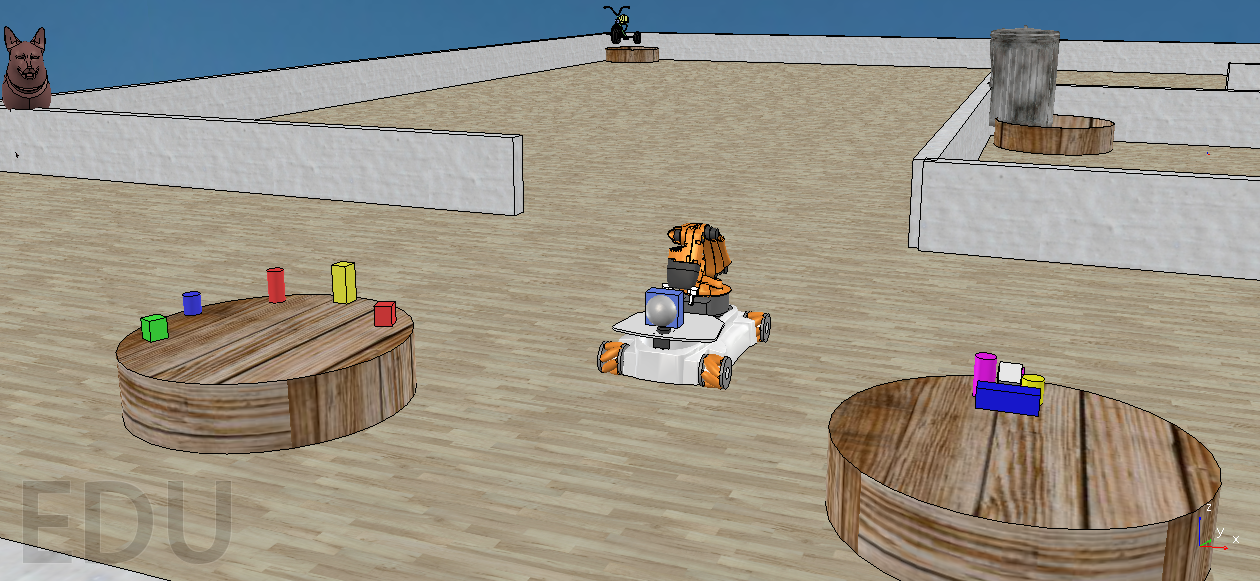
\includegraphics[width=1.00\textwidth]{starting_position.png}
	\caption{Example of a youBot starting position and its environment}
	\label{youbotStart}
\end{figure}

\FloatBarrier

\section{Implemented solutions}

\subsection{Map exploration}
\paragraph{}
The youBot stores a matrix representing the map. The elements of this matrix can have three different values. One value represents the fact that a cell of the map hasn't been explored yet, another means that it has been, and the last one implies the presence of an obstacle in the cell. During its exploration, the youBot can thus gather the data supplied by its Hokuyo sensors and update the values of this matrix easily because it knows its accurate postion in the map.   

\paragraph{} 
Now that we've explained how the youBot represents and updates its map, it remains to describe how the youBot will achieve to explore its environment entirely. Our exploration algorithm is the following:

\begin{enumerate}
\item The youBot rotates around itself in order to get a $360^{\circ}$ view of the map

\item The youBot selects the nearest unexplored point and establishes the trajectory to reach it

\item The youBot follows the trajectory, updates the map at the same time and makes sure that it's not running into an obstacle that wasn't yet acknowledged when the trajectory was established, otherwise, it goes back to step 2.

\item When the youBot reached his goal, \\if there is still unexplored points on the map: it goes back to step 2 \\else: the hole map has been explored.

\end{enumerate}



\subsection{Trajectories}

\paragraph{}
The trajectories of the youBot are calculated thanks to the (partial) map and the distance transform function from Peter Corke's robotics toolbox\cite{CorkeRTB}. A trajectory is an ordered list of points through which the youBot has to go. The more points the trajectory contains, the more fluid the trajectory is, so, based on the fluidity or precision we want to have, we can increase the number of points of a trajectory. 

\paragraph{}
To make the robot follows a trajectory, we used similar controllers to the ones presented in section 4.2.3 of Peter Corke's book "Robotics, vision and control"\cite{CorkeBook}. These controllers allows us to define a global velocity and a rotation velocity at each timestep but, in addition to that, we took advantage of the omnidirectional wheels of the youBot and turned the global velocity into a velocity vector, which components are the left-right and the forward-back velocities, as shown on figure \ref{velocities}.

\begin{figure}[h]
	\centering
		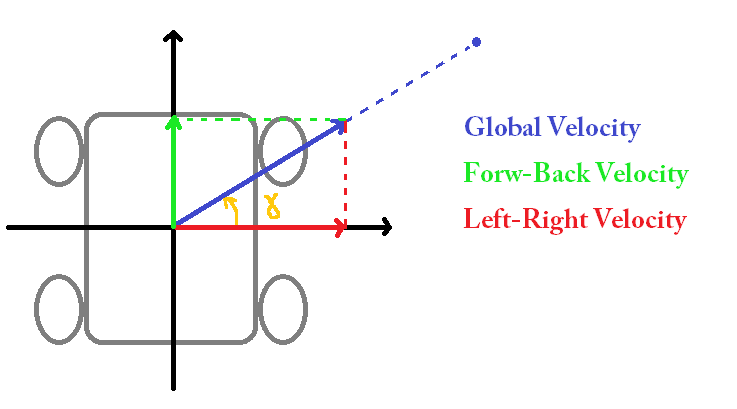
\includegraphics[width=10cm]{velocities.png}
	\caption{youBot omnidirectional velocity vector}
	\label{velocities}
\end{figure}

\FloatBarrier

\subsection{Locating and identifying baskets}

\paragraph{}


\subsection{Moving objects}

\paragraph{} 
The process that we've implemented to achieve this purpose is the following:
\begin{enumerate}
\item The youBot goes to the area of the table. This is done by defining some points that are at a certain distance around the table, and selecting the closest one as a goal.
\item When it reached this goal, the youBot rotates in order to position itself with its direction perpendicular to the line going through its center and the center of the table. There is however two directions that follow this criteria, so we chose the one that is pointing in the clockwise direction around the table (see figure \ref{tangent}).
\item The youBot then get close to the table using left-right velocity only.
\item When it is close enough, it takes a single 3D image with a large angle of view to detect objects above the table. Only the points that are above the table, and in a certain range, are kept.
\item Whether objects are detected or not, every moves that the youBot will make at this step and the three next ones will follow a circular path defined around the table. If nothing is detected, the youBot goes a bit further and starts again from step 4, unless this has been repeated enough times to make a complete turn of the table and realize that there is no object left on it. In that case the job is done. If, however, the 3D image contains any points, the youBot selects the closest one and moves to align its camera with that point and the center of the table.
\item The camera is oriented to the center of the table and takes, once again, a single 3D image, but this time with a shorter angle of view, and a small range, in order to see only one object.
\item The youBot then projects the points of this 3D image in the plane of the table and uses an implementation of the RANSAC algorithm\cite{RANSAC} to recognize circles of a given radius. If there is a match, the youBot then knows that the object is cylindrical but also knows the position of the center of this cylinder. If there is no match, the object is then box-shaped and each coordinate of the center of the box can be approximated by taking the extreme values and calculating their mean. 
\item The youBot moves to align its arm reference point with the center of the object and the center of the table.
\item The youBot places its arm tip in front of the box using V-REP IK.
\item It moves its arm slowly along a straight line trajectory going through the center of the object, still using V-REP IK, and then grab it.
\item The youBot then moves its arm to a configuration where the object will be just above the youBot platform and near the camera, so that it can take an RGB picture and guess the color of the object in the gripper. This guessing is performed by looking at only one particular point of the picture that is supposed to always belong to the object. It can lead to an unexpected color if the youBot somehow failed to grab anything and in that case, it goes back to step 4.   
\item The youBot moves its arm to its transport configuration, with the object still into the gripper, and goes to the appropriate basket to throw it. Then it goes back to step 1. Going to the baskets and getting close to them is performed with the same technique as for a table.

\end{enumerate}

\begin{figure}[h]
	\centering
		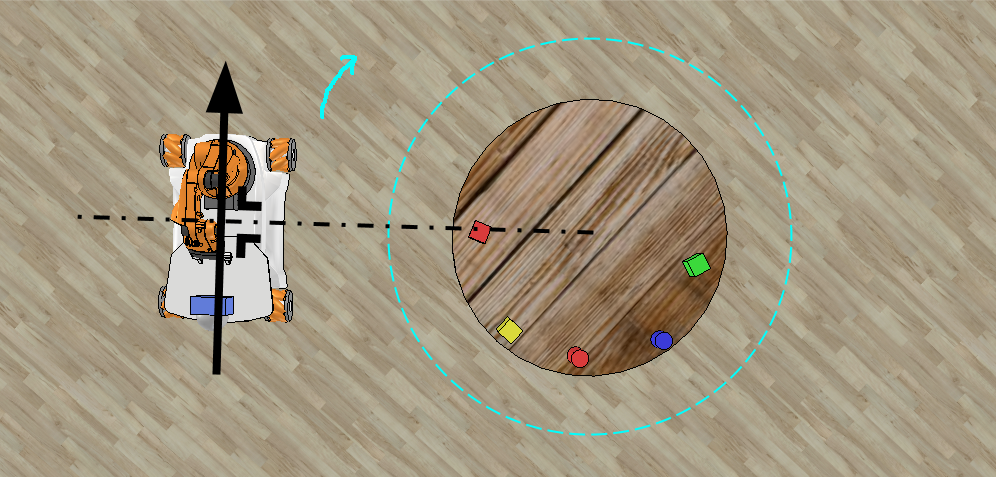
\includegraphics[width=1.00\textwidth]{tangent.png}
	\caption{youBot position before getting closer to the table}
	\label{tangent}
\end{figure}

\clearpage
\begin{thebibliography}{9}

\bibitem{trs}
Detry, Renaud. "Project definition" \textit{TRS: An Open-source Recipe for Teaching/Learning Robotics with a Simulator}. \\
\url{http://ulgrobotics.github.io/trs/project.html}

\bibitem{CorkeBook}
Corke, Peter. \textit{Robotics, Vision \& Control.} 2011.\\
\url{http://www.petercorke.com/RVC/}

\bibitem{CorkeRTB}
Corke, Peter. \textit{Robotics Toolbox for MATLAB}. Release 9. \\
\url{http://www.petercorke.com/Robotics_Toolbox.html}

\bibitem{RANSAC}
Zuliani, Marco. \textit{RANSAC toolBox.} \\
\url{https://github.com/RANSAC/RANSAC-Toolbox}


\end{thebibliography}

\end{document}